%% Requires compilation with XeLaTeX or LuaLaTeX
\documentclass[10pt,xcolor={table,dvipsnames},t]{beamer}
\usetheme{UCBerkeley}

\title[Your Short Title]{Introduction à la rétro-ingénierie}
\subtitle{Analyse statique et dynamique}
\author{Alexandre-Xavier Labonté-Lamoureux}
\institute{Délégation des compétitions en informatique de l'ÉTS}
\date{21 août 2019}

% numéros de page
%\sepackage{fancyhdr}
%\pagestyle{fancy}
%\fancyhf{}
%\rfoot{Page \thepage \hspace{1pt} of \pageref{LastPage}}
% fin numéros de page

\begin{document}

\section{Page titre}

{
    %\usebackgroundtemplate{%
    %    
\includegraphics[width=\paperwidth,height=\paperheight]{DeepDive_1024x683}}

    \begin{frame}
        \titlepage
    \end{frame}
}

% Uncomment these lines for an automatically generated outline.
%\begin{frame}{Outline}
%  \tableofcontents
%\end{frame}

\section{Introduction}

\begin{frame}{Planification de la séance}
    Contenu de la présentation
    \begin{itemize}
        \item La rétro-ingénierie
        \item Outils d'analyse
        \item Représentation des données
        \item Principes de l'analyse statique
        \item L'assembleur x86-64
        \item Principes de l'analyse dynamique
        \item Techniques anti-débogueur
        \newline
    \end{itemize}
À la suite de la présentation, il y aura un exercice à réaliser avec IDA Free.

%\begin{block}{}
%Nous verrons les outils suivants: Radare2 (snowman) avec Cutter, GDB (+ peda) ou pwngdb, Delvin, Compiler Explorer, IDA
%\newline
%\newline
%Chaque section sera suivie d'un exercice
%\end{block}

\end{frame}

\begin{frame}{La rétro-ingénierie}
    Pourquoi la rétro-ingénierie?
    \begin{itemize}
        \item Comprendre comment les programmes compilés fonctionnent à l'interne
        \item Être capable de réparer ses problèmes plus facilement avec un débogueur
        \item Comprendre les optimisations faites au code C et C++ par un compilateur
        \item Examiner un logiciel propriétaire pour en produire une version ouverte
        \item Récupérer le code source d'un logiciel dont on l'a perdu
        \item Étudier des logiciels malveillants et découvrir leurs propriétaires
        \item Espionnage industriel et vol de propriété intellectuel (déconseillé)
        % c'est vraiment pas nice, feke faites pas ça
        \newline
    \end{itemize}
    Cet atelier vise à vous donner une base qui vous rendra la rétro-ingénierie plus accessible.
\end{frame}


\begin{frame}
    \frametitle{Outils}
    
    \begin{columns}[T]
    
        \begin{column}{0.48\textwidth}
        GNU/Linux
        \begin{itemize}
            \item radare2 (avec Cutter), Ghidra
            \item GDB (avec plugin Pwngdb)
            \item Okteta Hex Editor
            \item \texttt{readelf}
            \item \texttt{strace}
            \item \texttt{ltrace}
            \item RetDec retargetable decompiler 
        \end{itemize}
        \end{column}
        
        \begin{column}{0.48\textwidth}
        Windows
        \begin{itemize}
            \item IDA Free
            \item x64dbg
            \item HxD Hex Editor
            \item PPEE (Professional PE file Explorer)
            \item WinDBG
            \item Sysinternals
            \item Snowman decompiler
        \end{itemize}
        \end{column}
    
    \end{columns}
\end{frame}


\begin{frame}
    \frametitle{Décompilateurs}
    
    \begin{columns}[T]
        \begin{column}{0.48\textwidth}
            \begin{itemize}
                \item RetDec retargetable decompiler 
                \item Snowman decompiler 
            \end{itemize}
        \end{column}
        \begin{column}{0.48\textwidth}
            \begin{itemize}
                \item Hex-Rays Decompiler
                \item JEB Decompiler \newline
            \end{itemize}
        \end{column}
    \end{columns}
    
    Pourquoi savoir lire l'assembleur quand on peut utiliser un décompilateur?
    
    \begin{itemize}
        % le code peut juste être optimizé et le décompilateur va mal fonctionner
        \item Les décompilateurs vont souvent générer du code inexacte.
        \item Les décompilateurs peuvent refuser de décompiler pour plein de raisons (instructions ou structure du programme invalides ou non reconnues)
        \item Les décompilateurs peuvent cacher des erreurs qu'on veut exploiter dans un programme.
        \item Certains programmes sont métas (auto-modification, introspection, etc.)
    \end{itemize}
    
\end{frame}


\section{Représentation des données}


\begin{frame}{Les fichiers exécutables}
    Connaissances à savoir pour effectuer la rétro-ingénierie. Il faut savoir que:
    \begin{itemize}
        \item Le code d'un exécutable est chargé tel quel en mémoire
        \item Il y a une \href{https://en.wikipedia.org/wiki/Relocation_(computing)}{relocalisation} si l'exécutable contient du «position-dependent code»
        % Avec GCC, on peut forcer noPIE, mais on a ne perte de performance de 10%
        \item Les exécutables ont une adresse de chargement préférée: 
        \begin{itemize}
            \item 0x00400000 (EXE, ELF/COFF), 0x10000000 (DLL), 0x0100 (COM)
        \end{itemize}
        \item Les EXE et DLL utilisent le format Portable Executable (PE) % Pour ELF c'est COFF
        \item Le code est dans un exécutable est sous forme d'opcodes (section \texttt{.text})
        \item Les opcodes peuvent être désassemblés
        \item Une instruction en assembleur est formée de un ou plusieurs opcodes
    \end{itemize}
\end{frame}

\begin{frame}{Encodage des instructions}
    Pour afficher les opcodes: Options $\rightarrow$ General $\rightarrow$ Number of opcode bytes
    \begin{figure}%\begin{center}
        %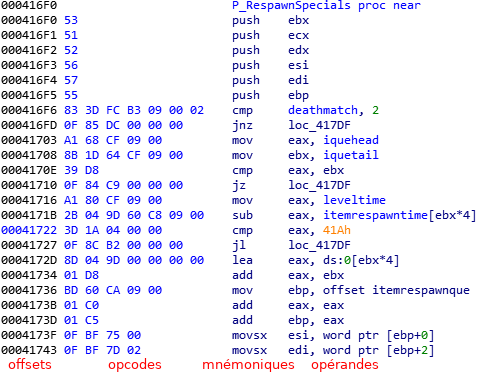
\includegraphics[width=.50\textwidth,height=.40\textheight]{Opcodes}
        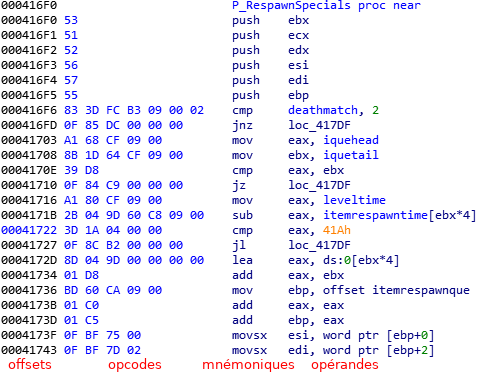
\includegraphics[width=0.58\textwidth]{Opcodes}
        %\caption{\label{fig:opcodes}Opcodes dans IDA représentés par des mnémoniques (offsets, opcodes, mnémoniques, opérandes)}
        % http://jargonf.org/wiki/mn%C3%A9monique
    \end{figure}

\end{frame}


% Partie 1 - L'analyse statique
\section{Analyse statique}

\begin{frame}{L'analyse statique}

\begin{itemize}
    \item Examen du code sans exécuter le programme.
    \item Pas besoin de tout comprendre: parfois on veut juste connaître les intrants ou extrants d'une fonction sans comprendre son fonctionnement.
    \item On a le droit de se fonder sur des suppositions et de poser des hypothèses.
    \item Pour les parties trop difficiles à comprendre d'un programme, se servir de l'analyse statique pour trouver où mettre des breakpoints et aller chercher les valeurs avec un débogueur. 
    \item Le but de la rétro-ingénierie, c'est d'en faire le moins possible.
\end{itemize}

%\begin{block}{Sous titre 2 genre}
%\end{block}

\end{frame}



\begin{frame}{Les registres du processeur}
    Voici un registre. Sur un processeur 64-bit, il peut contenir 8 octets. 
    
    Sur un processeur 32-bit, un maximum de 4 octets. 
    
    \begin{center}
    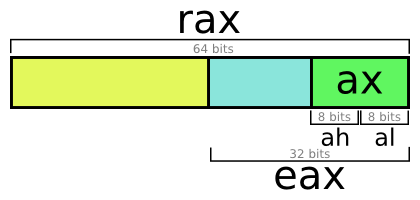
\includegraphics[width=.60\textwidth,height=.40\textheight]{Register}\newline{}
    Source: \href{http://blog.jpauli.tech/2016-11-30-on-c-performances-html/}{Registers}
    \end{center}
\end{frame}

\begin{frame}{Les registres du processeur}

    \begin{center}
    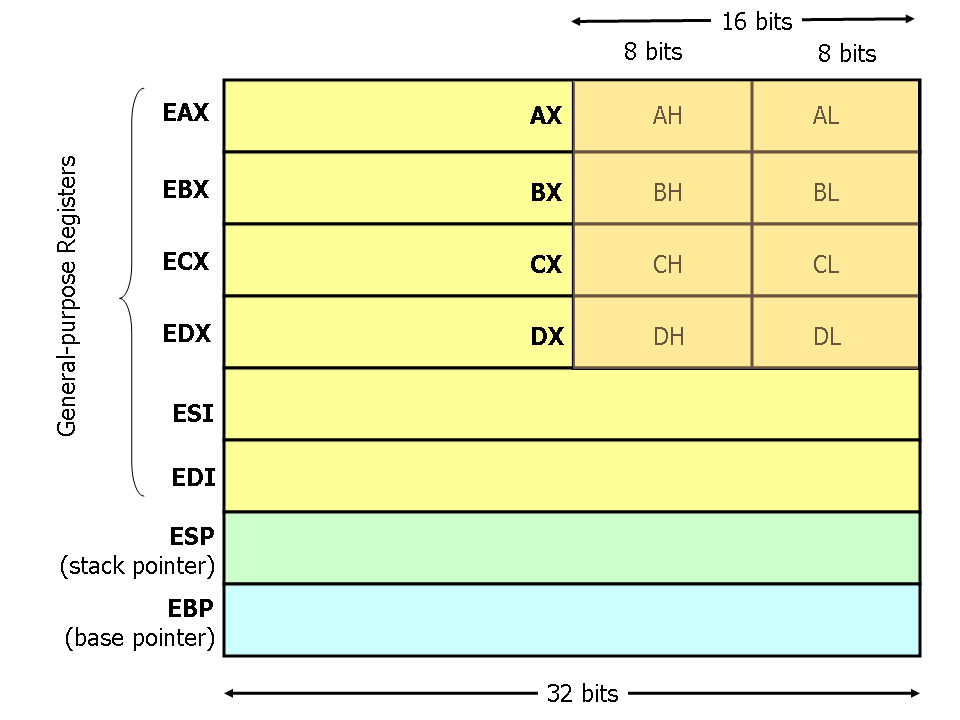
\includegraphics[width=.60\textwidth,height=.60\textheight]{x86-registers}\newline{}
    Source: \href{https://www.cs.virginia.edu/~evans/cs216/guides/x86.html}{Registers}
    \end{center}
\end{frame}

\begin{frame}{Flags de processeur}
    \begin{itemize}
        \item Il y a un registre FLAGS (EFLAGS sur 32-bit, RFLAGS sur 64-bit). 
        \item Il sert à conserver le résultat des conditions rencontrées dans le code.
        \item Les «flags» sont modifiés par certaines instructions. Ils affectent le flot d'exécution du code (instructions de type «jump» conditionnel).
        \item Ils sont modifiés par les instructions comme \texttt{cmp}, mais peuvent aussi être modifiés par des instructions comme \texttt{sub} ou \texttt{dec}. 
        \item Il n'est pas utile de les connaître pour faire la rétro-ingénierie.
    \end{itemize}
\end{frame}


\begin{frame}{La pile (stack)}

La pile est un mécanisme LIFO utilisé pour préserver des données lors des changements de portée («scope»). Ex: lorsqu'on entre dans une fonction.

\begin{center}
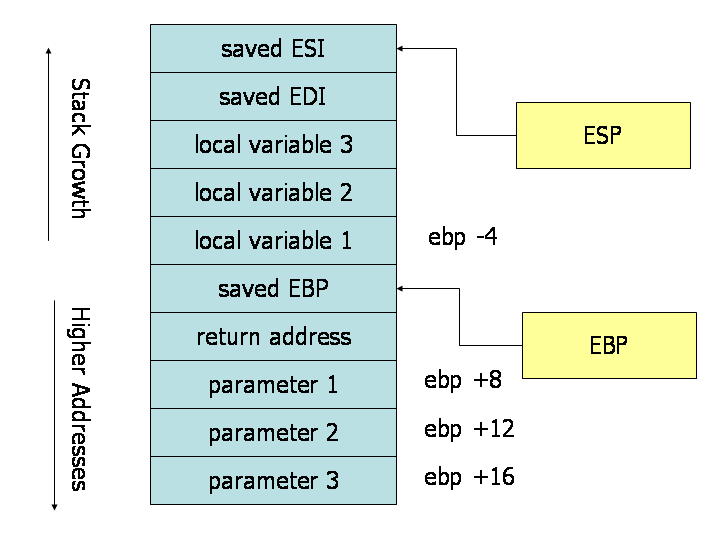
\includegraphics[width=.60\textwidth,height=.56\textheight]{Stack-convention}\newline{}
Source: \href{https://www.cs.virginia.edu/~evans/cs216/guides/x86.html}{x86 Assembly Guide}
\end{center}

\end{frame}


\begin{frame}{Conventions d'appel}
    \begin{itemize}
        \item Définit l'ordre d'empilage des paramètres à passer à une fonction.
        \item Définit qui doit dépiler ces paramètres. 
        \item Ces conventions sont \texttt{cdecl}, \texttt{stdcall}, \texttt{fastcall}, etc.
        \item La convention varie selon le compilateur et les conventions peuvent changer à l'intérieur d'un même programme.
        \item Pour plus d'info: \href{https://en.wikipedia.org/wiki/X86_calling_conventions}{x86 calling conventions}
    \end{itemize}
\end{frame}

\begin{frame}{Conventions d'appel: Dans le cas de GCC}
    \begin{itemize}
        \item GCC utilise \texttt{cdecl}. Les paramètre sont passés de droite à gauche.
        \item Exemple: Retour dans \texttt{eax}, paramètres dans \texttt{edi}, \texttt{esi}, \texttt{edx}, \texttt{ecx}:
        
        \begin{center}
            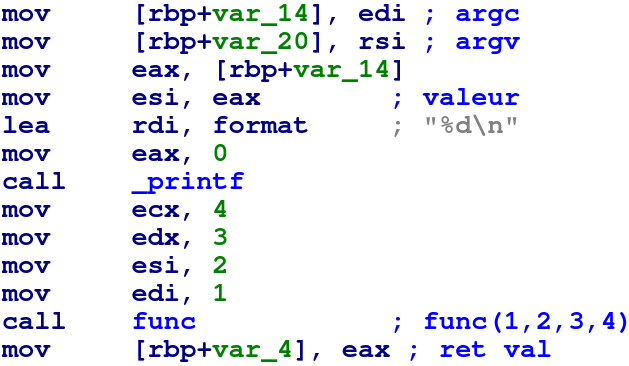
\includegraphics[width=.60\textwidth,height=.55\textheight]{appels}
        \end{center}
    \end{itemize}
\end{frame}



%\section{Some \LaTeX{} Examples}

\begin{frame}
    \frametitle{Boutisme (Endianness)}
    Représentation des données en mémoire. L'ordre des octets change.
    \begin{columns}[T]
        \begin{column}{0.48\textwidth}
            Gros-boutisme (Big-endian)
            % l'octet ayant le poids le plus fort est enregistré en premier
            \begin{itemize}
                \item Les protocoles TCP/IP 
                \item PCI Express
                \item Java
            \end{itemize}
        \end{column}
        
        \begin{column}{0.48\textwidth}
            Petit-boutisme (Little-endian)
            % network byte order
            \begin{itemize}
                \item Processeurs Intel et ARM
                \item 0xA0B70708 est représenté en mémoire comme \texttt{08 07 B7 A0}
            \end{itemize}
        \end{column}
        % bi-boutisme et mi-boutisme c'est de l'hérésie
    \end{columns}
    
    \begin{center}
    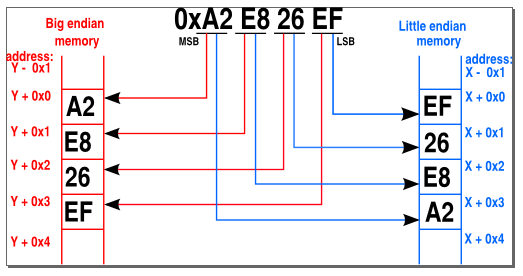
\includegraphics[width=.56\textwidth,height=.4\textheight]{Page-2-Image-3.png}%\newline{}
%Source: \href{https://www.nxp.com/docs/en/application-note/AN4657.pdf}{Comparison of Big-Endian Versus Little-Endian}
    \end{center}
\end{frame}


%\subsection{Instructions les plus communes en assembleur}
\section{Survol de l'assembleur x86-64}

%\smallframetitle
\normalframetitle

\begin{frame}{Transfert de données}

    \begin{table}
    \centering
    \begin{tabular}{c c}
    \tableheadrow
    \tableheadcol{Instruction} & \tableheadcol{Effet} \\
    \texttt{mov dst, src} & dst = src (copie) \\
    \texttt{xchg dst1, dst2} & Échange dst1 et dst2 \\
    \texttt{push src} & push src, décrémente rsp \\
    \texttt{pop dst} & pop dst, décrémente rsp
    \end{tabular}
    \caption{\label{tab:instrans}Instructions de transfert de données}
    \end{table}
\end{frame}

\begin{frame}{Opérations arithmétiques}
    \begin{table}
    \centering
    \begin{tabular}{c c}
    \tableheadrow
    \tableheadcol{Instruction} & \tableheadcol{Effet} \\
    \texttt{add dst, src} & dst += src \\
    \texttt{sub dst, src} & dst -= src \\
%    \texttt{mul src} & eax *= src \\
%    \texttt{div src} & eax /= src \\
    \texttt{inc dst} & dst += 1 \\
    \texttt{dec dst} & dst -= 1 \\
    \texttt{neg dst} & dst = -dst \\
    \texttt{cmp src1, src2} & src1 - src2: Change le status flag
    \end{tabular}
    \caption{\label{tab:insarith}Instructions pour les opérations arithmétiques}
    \end{table}
\end{frame}

\begin{frame}{Opérations logiques et «bitwise»}
    Bitwise operations: Opérations au niveau du bit.
    \begin{table}
    \centering
    \begin{tabular}{c c}
    \tableheadrow
    \tableheadcol{Instruction} & \tableheadcol{Effet} \\
    \texttt{and dst, src} & dst \&= src \\
    \texttt{or dst, src} & dst |= src \\
    \texttt{xor dst, src} & dst \textasciicircum= src \\
    \texttt{not dst} & dst = \textasciitilde dst \\
    \texttt{test src1, src2} &  src1 \& src2: Change le status flag
    \end{tabular}
    \caption{\label{tab:insbitwise}Instructions pour les opérations logiques et les opérations sur les bits}
    \end{table}
    
    Opérations «Shift» et «Rotate»: \href{https://en.wikibooks.org/wiki/X86_Assembly/Shift_and_Rotate}{\texttt{X86 Assembly/Shift and Rotate}}
\end{frame}

\begin{frame}{Instructions pour les sauts conditionnels}
    % Les instructions de type JMP conditionnels suivent souvent l'instruction CMP, mais pas tout le temps. 
    Non signé: above/below\newline
    Signé: greater/lower
    
    Bonne lecture: 
    \href{https://www.tutorialspoint.com/assembly_programming/assembly_conditions.htm}{\texttt{Assembly - Conditions}}
    
    \begin{table}
    \begin{center}
    \begin{tabular}{ c c c }
        \tableheadrow
        \tableheadcol{Type} & \tableheadcol{non signé} & \tableheadcol{signé} \\
        == & JE/JZ & JE/JZ \\
        != & JNE/JNZ & JNE/JNZ \\
        > & JA/JNBE & JG/JNLE \\
        >= & JAE/JNB & JGE/JNL \\
        < & JB/JNAE & JL/JNGE \\
        <= & JBE/JNA & JLE/JNG
    \end{tabular}
    \end{center}
    \caption{\label{tab:inscondjmp}Sauts conditionnels}
    \end{table}
\end{frame}

\begin{frame}{Instructions pour les sauts conditionnels}
    Les instructions de type JMP conditionnel suivent souvent l'instruction CMP ou TEST, mais pas tout le temps. Les sauts se fient aux flags, mais ceux-ci peuvent être modifiés autrement. Voir \href{http://unixwiz.net/techtips/x86-jumps.html}{ici} pour les flags.
    \newline{}\newline{}
    Exemple de jump dans une fonction en assembleur (var\_4 = -4 sur le stack):
    
    \begin{center}
    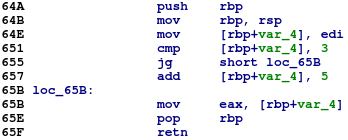
\includegraphics[width=.65\textwidth,height=.42\textheight]{Ex_jump}
    \end{center}
\end{frame}

\begin{frame}{Branches non-conditionnelles}
    Régule le flot d'exécution (code flow)
    \begin{table}
    \centering
    \begin{tabular}{c c}
    \tableheadrow
    \tableheadcol{Instruction} & \tableheadcol{Effet} \\
    \texttt{jmp addr} & Sauter à un adresse \\
    \texttt{call addr} & Push retaddr, saute à l'adresse \\
    \texttt{ret} & Pop retaddr, saute à son adresse \\
    \texttt{syscall} & Appelle le kernel
    \end{tabular}
    \caption{\label{tab:insbranch}Instructions pour les branches non-conditionnelles}
    \end{table}
\end{frame}

\begin{frame}{Autres instructions}
    \begin{table}
    \centering
    \begin{tabular}{c c}
    \tableheadrow
    \tableheadcol{Instruction} & \tableheadcol{Effet} \\
    \texttt{lea dst, src} & Charge l'adresse mémoire dans dst \\
    \texttt{nop} & Fait rien (opcode: 0x90)
    \end{tabular}
    \caption{\label{tab:insother}Autres instructions}
    \end{table}
\end{frame}

%\subsection{Patterns}
\section{Patterns communs et code obscurci}

\begin{frame}{Instruction XOR}
    Opération XOR telle que l'opérateur \texttt{\textasciicircum}
    \begin{itemize}
        \item \texttt{xor eax, eax} pour mettre le registre EAX à zéro
        \item L'opération XOR dans des boucles peut indiquer qu'il y a encodage
        \item Menu \texttt{Search} -> \texttt{Text}, entrez «xor», puis \texttt{Search all occurrences}
        \item NULL-preserving XOR: Ne XOR pas les 0 ou les valeurs qui sont == à la clef
    \end{itemize}
    
        \begin{columns}[T]
    
        \begin{column}{0.48\textwidth}
        XOR
        \begin{itemize}
            \item \texttt{buf[i] \textasciicircum= key;}
        \end{itemize}
        \end{column}
        
        \begin{column}{0.48\textwidth}
        NULL-preserving XOR
        \begin{itemize}
            \item \texttt{if(buf[i]!=0 \&\& buf[i]!=key)}
            \item \texttt{\quad buf[i] \textasciicircum= key;}
        \end{itemize}
        \end{column}
    
    \end{columns}
    
\end{frame}

\begin{frame}{String stacking}
    Caractères empilés sur la pile. La \href{http://www.asciitable.com/}{table ASCII} est votre ami!
    \begin{itemize}
        \item Sous forme de caractères: Quand c'est une suite de caractères, on peut les convertir en un seul string. 
        \item Sous forme d'entiers: Quand c'est des nombres, on peut les convertir en chaînes de caractères et elles seront affichées à l'envers.
    \end{itemize}

    \begin{center}
        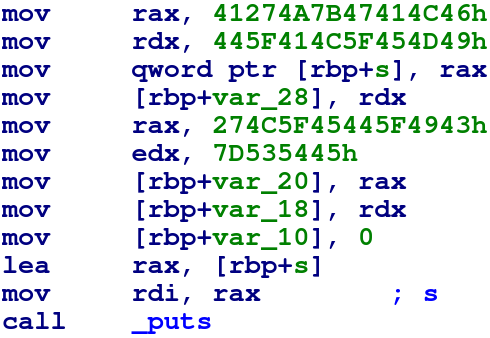
\includegraphics[width=.44\textwidth,height=.46\textheight]{stringstack}
    \end{center}

\end{frame}

\begin{frame}{Programmes cachés}
    Il y a plusieurs façon de cacher un programme dans un autre pour compliquer l'analyse. Le programme principal sert donc qu'à en faire son extraction.
    
    Quelques exemples de programmes cachés:
    \begin{itemize}
        \item Sous forme de shellcode, injecté dans un autre processus ou non.
        \item Intégré à la section \texttt{.rsrc} d'un PE ou embarqué dans un ELF
        \item Compressé (UPX, aPACK) ou packé avec un algorithme de chiffrement/obfuscation (PECompact, ASPack, Armadillo)
        \item Fichier exécutable compressé avec des algorithmes du Windows API \href{https://docs.microsoft.com/en-us/windows/win32/cmpapi/-compression-portal}{(voir MSDN)} et injecté dans un autre processus.
        \item \href{https://www.exetools.com/}{\texttt{https://www.exetools.com/}}
    \end{itemize}
\end{frame}


\begin{frame}
    \frametitle{Techniques anti-désassembleur}
    Ces techniques visent à induire le désassembleur en erreur afin qu'il nous affiche les mauvaises instructions.
    
    Le désassembleur ne fait pas la différence entre des instructions et des données.
    \begin{itemize}
        \item Ex: Call pour sauter par dessus le texte «hello». 
        
        \texttt{E8 06 00 00 00 68 65 6c 6c 6F 00 58 C3}
    \end{itemize}
    
    Il est aussi possible d'utiliser les instructions jump pour rendre le désassemblage impossible.
    \begin{itemize}
        \item Ex: Instruction JMP relatif qui saute à l'intérieur de ses propres opcodes
        
        \texttt{EB FF C0 FF C8}
    \end{itemize}
\end{frame}


\section{Analyse dynamique}

\begin{frame}
    \frametitle{Analyse dynamique}
    \begin{itemize}
        \item On exécute le programme afin de voir ce qu'il fait.
        \item On peut utiliser un débogueur pour voir ce qu'il se passe à l'intérieur.
        \item Complémentaire à l'analyse statique quand on veut aller chercher quelles sont les valeurs de certaines variables dans le code.
    \end{itemize}

\end{frame}



\begin{frame}
    \frametitle{Interception de données (Linux)}

    \begin{itemize}
        \item \texttt{ltrace} (Library call tracer)
        \begin{itemize}
            \item Capture les appels entre le programme étudié et les bibliothèques partagées
            \item \texttt{ltrace -e 'str*' ./flagcmp}
        \end{itemize}
        \item \texttt{strace} (System call tracer)
        \begin{itemize}
            \item Capture les appels entre le programme étudié et le noyau Linux
            \item \texttt{strace -e trace=open,read ls /home}
        \end{itemize}
        \item \texttt{LD\_PRELOAD}
        \begin{itemize}
            \item On s'en sert pour détourner des appels à des fonctions de bibliothèques partagées vers nos propres fonctions. 
            \item \texttt{LD\_PRELOAD=./libnosleep.so ./slow\_program}
        \end{itemize}
    \end{itemize}

\end{frame}

\begin{frame}
    \frametitle{Techniques anti-débogueur}
    Techniques qui permettent à un programme de savoir s'il se fait déboguer
    
    \begin{itemize}
        \item \texttt{ptrace} (Appel système Linux)
        \begin{itemize}
            \item Permet à un processus d'en contrôler un autre. Un processus peut se faire contrôler par un seul processus à la fois.
        \end{itemize}
        
        \item Lancer des signaux
        \begin{itemize}
            \item Un programme peut définir ses propres gestionnaires de signaux
            \item Si le programme s'exécuter dans un débogueur, le débogueur attrapera les signaux à sa place.
            \item Un programme peut implémenter son propre gestionnaire de breakpoints
        \end{itemize}
        
        \item Détection de breakpoints
        \begin{itemize}
            \item Un programme peut faire un \textit{checksum} de sa mémoire pour détecter des modifications. Un breakpoint place un \texttt{0xCC} en mémoire.
        \end{itemize}
        
    \end{itemize}
\end{frame}



\section{Analyse avec IDA}

\begin{frame}{IDA}

    \begin{itemize}
        \item Logiciel de rétro-ingénierie qui permet de désassembler des programmes
        \item IDA Pro est le gold standard, mais peut coûter environ \$3000
        \item IDA Free, une version Freeware existe: \href{https://www.hex-rays.com/products/ida/support/download_freeware.shtml}{téléchargez-là ici} 
        \item Permet de visualiser l'assembleur et le code flow dans un graphique
        \item Permet de sauvegarder notre travail dans une base de données
        \item La version payante permet d'écrire des scripts Python, de décompiler du code et supporte plusieurs architectures CPU différentes.
    \end{itemize}
\end{frame}


\begin{frame}{Raccourcis dans IDA}
    Cliquer pour placer le curseur à un endroit approprié, puis appuyer...
    \begin{itemize}
        \item \texttt{U}: Indéfinir une donnée
        \item \texttt{A}: Convertir en string
        \item \texttt{D}: Convertir en donnée
        \item \texttt{C}: Convertir en code
        \item \texttt{R}: Convertir en caractère
        \item \texttt{:} et \texttt{;} : Mettre un commentaire
        \item \texttt{X}: Pour trouver les références croisées
        \item \texttt{N}: Renommer une fonction ou une variable
        \item \texttt{«espace»}: Alterner entre la vue «Graph» et «Text»
    \end{itemize}
\end{frame}


\begin{frame}{Modifier un programme dans IDA}
    Dans le menu Edit $\rightarrow$  Patch program
    \begin{itemize}
        \item \texttt{Change byte}: Utile pour modifier jusqu'à 16 opcodes à la fois (pour les NOPer par exemple)
        \item \texttt{Change word}: Pour modifier 16 bits
        \item \texttt{Assemble}: Permet d'écrire de l'assembleur à insérer dans le code (attention: les instructions ont différentes tailles!)
    \end{itemize}
    
    Notez que IDA n'a pas de fonction «undo», donc faites attention à ce que vous faites. Sauvegardez souvent pour pouvoir retourner à un état précédant.
\end{frame}


\section{Atelier}

\begin{frame}{Méthodologie}
    \begin{itemize}
        \item Privilégier l'analyse statique
        \item Se servir de l'analyse dynamique que pour confirmer la compréhension de la rétro-ingénierie par analyse statique
        \item Ne pas modifier le binaire
        \item Toujours commencer avec les commandes \texttt{strings} ou \texttt{binwalk} parce qu'elles peuvent révéler des informations qu'on pourrait passer à côté autrement
    \end{itemize}
    
    \begin{block}{«Ouin mais reverser l'assembleur c'est tough»}
        Plus t'en fait, plus tu deviens bon!  ;-)
    \end{block}
\end{frame}


\begin{frame}{À garder en tête}
    Parfois, on semble manquer d'information durant la rétro-ingénierie et le code peut être difficilement compréhensible. 
    \begin{itemize}
        \item Faire des déductions
        \begin{itemize}
            \item Ne pas hésiter à émettre des hypothèses
            \item Se servir de son instinct de programmeur
        \end{itemize}
        \item Document son travail
        \begin{itemize}
            \item Mettre des commentaires dans le code et y revenir plus tard
            \item Renommer les fonctions pour indiquer ce qu'elles font
        \end{itemize}
        \item Écrire du pseudocode afin de s'aider à comprendre
        \item Ne pas perdre son temps à essayer de comprendre des instructions qui n'ont pas un impact sur le calcul qui est fait (souvent \texttt{rbp} et \texttt{rsp})
    \end{itemize}
\end{frame}


\begin{frame}{Défi}
    Effectuez la rétro-ingénierie d'un binaire avec \href{https://www.hex-rays.com/products/ida/support/download_freeware.shtml}{IDA Free} afin de comprendre son fonctionnement au complet.
    \begin{itemize}
        \item Identifiez les changements que le programme fait à l'ordinateur
        \item Pouvez-vous trouver: 
        \begin{itemize}
            \item Deux buffer overflows?
            \item Une race condition?
            \item Un autre bug?
        \end{itemize}
        \item Codez un extracteur qui décode ce que le programme contient
    \end{itemize}
    %Il est défendu d'utiliser un autre logiciel que IDA Free pour faire le défi!
    Mettez vous en équipe de deux pour ne pas souffrir seul dans votre coin!
\end{frame}


\normalframetitle

\iffalse

% Autres défis à faire
\section{Autres défis à faire}

\begin{frame}{CTF101, Montré-Hack, avril 2019}
    \begin{itemize}
        \item Temps estimé: 40 minutes
        \item Essayez l'analyse statique et l'analyse dynamique pour résoudre le défi
        \item Il y a un bug dedans, pouvez-vous le trouver?
        \item Instruction \texttt{gle \$a \$b} bébitte chat.
    \end{itemize}
    
    \begin{block}{Solution (cachée)}
        \begin{itemize}
            \item Trouver la fonction SHA et déterminez ce qu'elle fait
            \item Patcher l'instruction signal avec NOP, sautez par dessus avec le débogueur ou ignorer les signaux avec \texttt{handle SIGSEV nostop}
        \end{itemize}
    \end{block}
\end{frame}

\begin{frame}{DCI CTF, septembre 2018}
    \begin{itemize}
        \item Temps estimé: 30 minutes
        \item Essayez l'analyse statique et l'analyse dynamique pour résoudre le défi
        \item Incide: Pourquoi le programme est-il lent?
    \end{itemize}
    
    \begin{block}{Solution (cachée)}
        \begin{itemize}
            \item Remplacer les instructions \texttt{sleep} par des \texttt{NOP}
        \end{itemize}
    \end{block}
\end{frame}

\begin{frame}{OWASP CTF, Hackfest, novembre 2018}
    \begin{itemize}
        \item Temps estimé: 20 minutes
        \item Utiliser \texttt{strings} and imprimer l'assembleur avec \texttt{radare}
        \item Résoudre le défi en observant les instructions assembleur et les appliquer sur le string trouvé
    \end{itemize}
    
    \begin{block}{Solution (cachée)}
        \begin{itemize}
            \item Facile
        \end{itemize}
    \end{block}
\end{frame}

\fi % \iffalse

\section{Ressources}

% Pour la suite %
\begin{frame}
    \frametitle{Ressources externes}
    \begin{itemize}
        \item Faire des défis sur \texttt{Root Me}: \url{https://www.root-me.org/en/Challenges/Cracking/}
        % url serait le lien complet, mais comme texture juste mettre le domaine
        \item Faire des défis sur \texttt{RingZer0}: \url{https://ringzer0ctf.com/challenges/}
        \item Pour s'habituer à lire l'assembleur et le comparer avec le code \texttt{C} correspondant: 
        \item Utile pour décoder plusieurs formats de données qu'on peut trouver dans un fichier exécutable: \url{https://gchq.github.io/CyberChef/}
    \end{itemize}
\end{frame}


% Références %
\section{Références}

\begin{frame}
    \frametitle{Références}
    \begin{itemize}
        \item Code source de cette présentation et des exercices: \url{https://github.com/AXDOOMER/WorkshopIntroRevEng}
        \item Inspiré par un ancien \href{https://dciets.com/dci-workshop/security/2017/09/13/re/}{workshop fait par Francis Labelle}
    \end{itemize}
    
    \begin{block}{Licence}
        Cette présentation est distribuée sous la licence 
        \href{https://creativecommons.org/licenses/by-nc-sa/4.0/deed.fr}{\texttt{CC BY-NC-SA 4.0}}.
        
        Les images tirées d'Internet restent la propriété de leur pripriétaire respectif. 
        
        Le modèle de cette présentation peut être trouvé 
        \href{https://www.overleaf.com/latex/templates/uc-berkeley-beamer-theme/bywswngntrws}{ici}.
        
        \begin{center}
            
\includegraphics[width=.20\textwidth,height=.10\textheight]{rect-by-nc-sa-300x105}
        \end{center}
    \end{block}
\end{frame}

\end{document}
